\chapter{TiveJS}
    In questo lavoro, come introdotto, presento TiveJS, che è un porting ed un'evoluzione di Tive e come esso è in grado di: permettere la progettazione di sentenze visive grazie all'ausilio di palette di simboli personalizzate, il riconoscimento di linguaggio diagrammatici e la traduzione di quest'ultimi.
    \newline
    Il paper da cui deriva questo lavoro è \textit{Using the local context for the definition and implementation of visual languages}~\cite{localcontext} in cui si parla di un metodo per la traduzione di diagrammi o in generale di sentenze visuali in sentenze semantiche.

    \section{Funzionamento e Implementazione}
        Il funzionamento si suddivide principalmente in tre fasi, mostrate schematicamente nella figura~\ref{fig:funzionamento}: la progettazione del diagramma, il riconoscimento di quest'ultimo e l'applicazioni delle definizioni sintattiche e semantiche. Durante tutte le procedure la navigazione all'interno del grafo viene effettuata attraverso delle espressioni chiamate SGPath.
        \newline
        \begin{figure}[htbp]
            \centering
            \smartdiagramset{border color=none,
                back arrow disabled=true,
                text width=3.5cm,
                module minimum width=3.5cm,
                module x sep=5
            }
            \smartdiagram[flow diagram:horizontal]{Progettazione, Riconoscimento, Applicazione Definizioni}
            \caption{Diagramma del funzionamento di TiveJS}
            \label{fig:funzionamento}
        \end{figure}

        Come vedremo, ogni fase può suddividersi in più sotto-fasi illustrate nel dettaglio nelle prossime sezioni.

        \subsection{SGPath}
            Questa sezione descrive una specifica simile a XPath\footnote{\textit{"In informatica XPath è un linguaggio, parte della famiglia XML, che permette di individuare i nodi all'interno di un documento XML. Le espressioni XPath, a differenza delle espressioni XML, non servono a identificare la struttura di un documento, bensì a localizzarne con precisione i nodi."} \cite{xpath}} per la navigazione del grafo chiamata SGPath. Mentre XPath definisce delle espressioni per la navigazione all'interno dei file XML, SGPath definisce delle espressioni per navigare in una struttura a grafo.
            \newline
            Un SGPath consiste di passaggi (o \textit{step}). Ogni passo è valutato su un insieme di nodi del grafo. Il risultato di ogni passo è un insieme di nodi del grafo. SGPath può far uso delle proprietà dei simboli quali nome, id, ecc.
            \newline
            La sintatssi di un SGPath è strutturata in questo modo:
            \begin{quotation}
                \textbf{sgpath\_step\_1/sgpath\_step\_2/ … /sgpath\_step\_n}
            \end{quotation}
            ogni sgpath\_step è formato in questo modo:
            \begin{quotation}
                \textbf{axis(edge-filter)::node-test[predicate]}
            \end{quotation}
            dove:
            \begin{itemize}
                \item \textbf{axis(edge-filter)::} è opzionale e indica come continuare la navigazione partendo dal nodo corrente. A differenza di XPath, concede di spostari solo tra nodi adiacenti.
                \item \textbf{node-test} indica il nodo da raggiungere. Può essere il nome di un elemento o * per indicare qualsiasi nodo.
                \item \textbf{\lbrack predicate\rbrack} è opzionale e permette di selezionare i nodi con attributi specifici.
            \end{itemize}
            Ecco alcuni esempi di SGPath:
            \begin{itemize}
                \item \textit{CON\_E\_A/KEY\_ATTR}
                \item \textit{CON\_E\_R[@Cardin='([01],N)']/ENTITY}
                \item \textit{(\#attName = 'Up')::ARROW/PRED}
            \end{itemize}
            In TiveJS l'algoritmo che si occupa della risoluzione degli SGPath è visibile all'interno dello snippet \ref{lst:resolvePath}. La funzione \texttt{resolvePath} divide la stringa al carattere '\texttt{/}' così da ottenere ogni step del percorso. A questo punto ogni step viene scorporato di tutti i suoi campi dalla funzione \texttt{scorporatePath} ottenendo un oggetto con all'interno tutte le informazioni sul singolo step.
            \begin{lstlisting}[language=JavaScript,caption=\textbf{Funzione che si occupa della risoluzione delle path},label={lst:resolvePath}]
                /**
                * Resolve path
                */
                CheckUtil.prototype.resolvePath = function (node, path) {
                    console.log('RESOLVING A PATH FOR: ' + node.id);
                    console.info('node, path', node, path);
                    let nodes = [];
                    nodes = nodes.concat(node);
                    let splittedPath = path.split('/');
                    for (let elem in splittedPath) {
                        let pathStep = splittedPath[elem];
                        nodes = this.resolvePathStep(nodes, pathStep);
                    }
                    console.info('returned nodes', nodes);
                    return nodes;
                }
            \end{lstlisting}
        
        \subsection{Progettazione di sentenze visive}
            La progettazione delle sentenze visive avviene attraverso una GUI\footnote{Interfaccia Grafica.} molto semplice ed intuitiva, simile a quella nella figura~\ref{fig:drawio}.

            \begin{figure}[htbp]
                \centering
                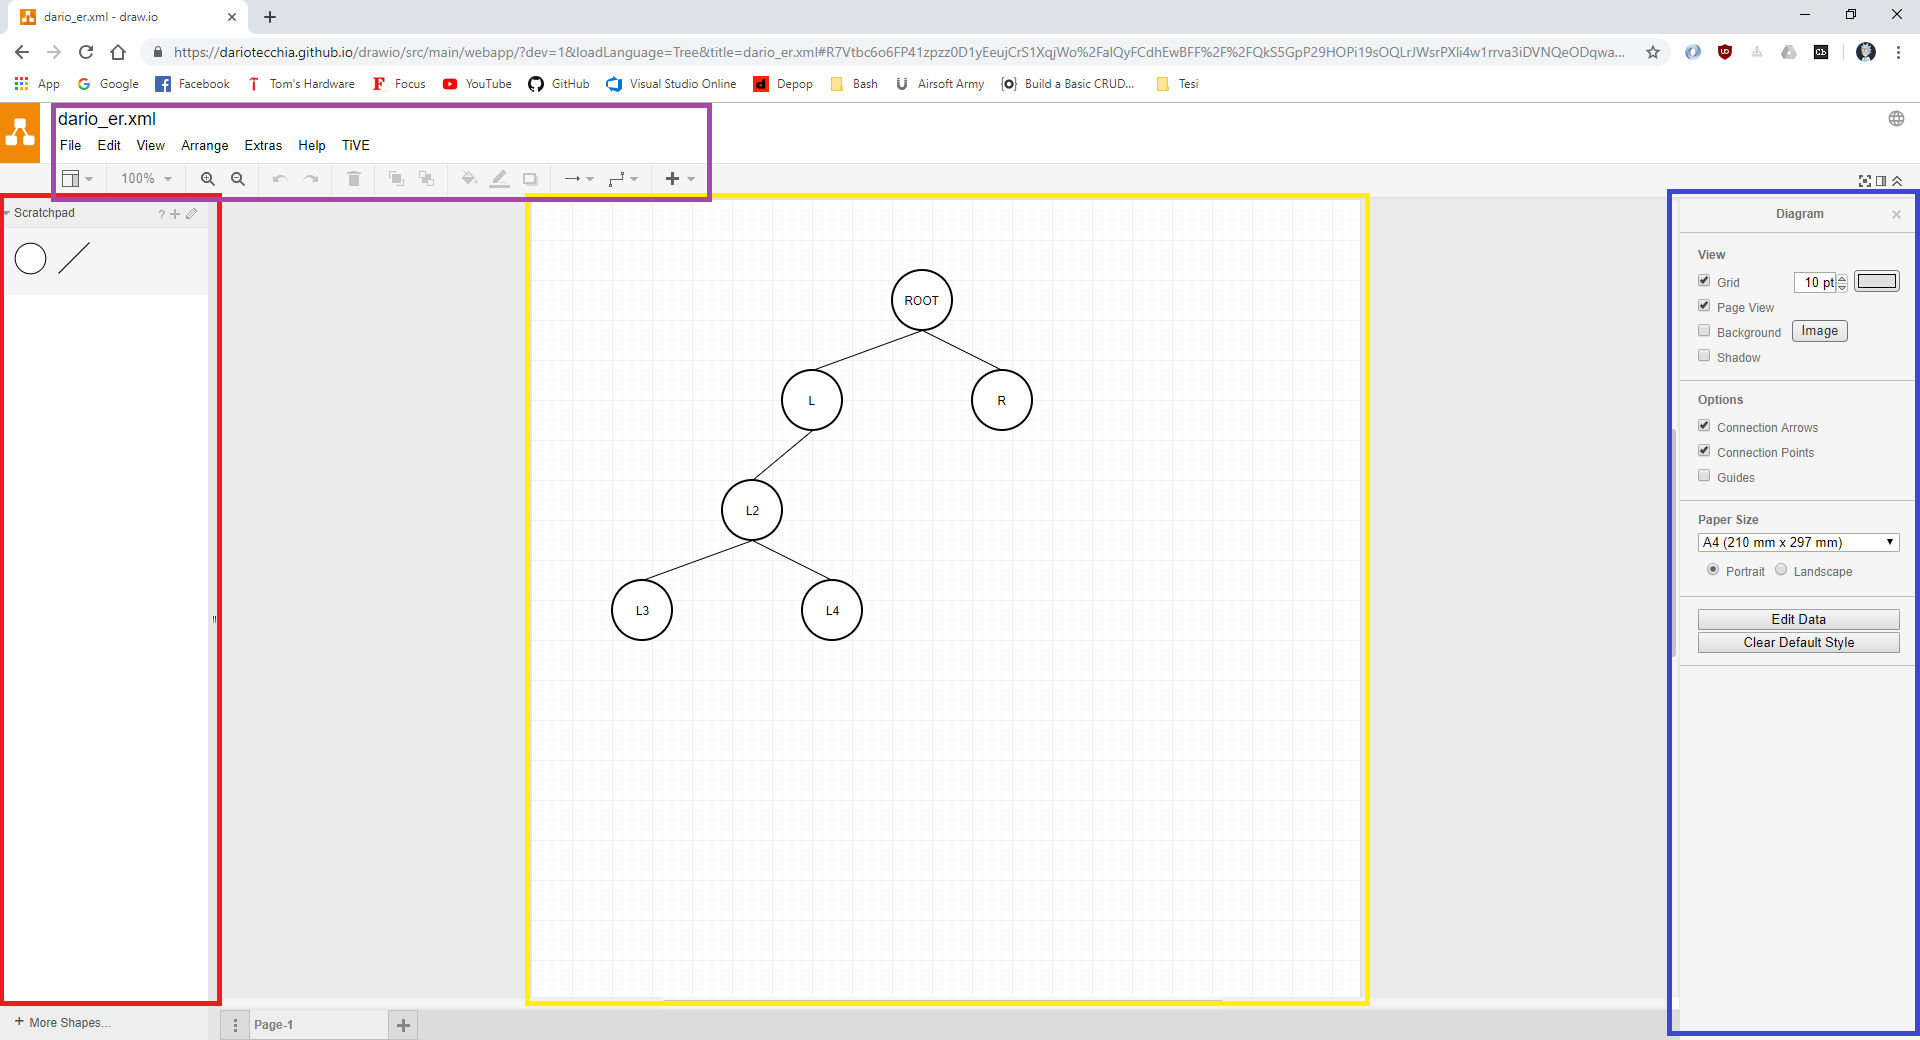
\includegraphics[scale=0.25]{Figure/tivejs_gui2.png}
                \caption{Schermata principale di TiveJS}
                \label{fig:tivejsgui}
            \end{figure}

            E' composta di quattro sezioni principali (figura~\ref{fig:tivejsgui}):
            \begin{itemize}
                \item Barra laterale sinistra (evidenziata \textcolor{red}{rosso})
                \item Barra laterale destra (evidenziata \textcolor{blue}{blu})
                \item Area di lavoro (evidenziata \textcolor{yellow}{giallo})
                \item Barra dei menu (evidenziata \textcolor{purple}{viola})
            \end{itemize}
            All'interno della barra laterale sinistra troviamo la palette dei simboli importata precedentemente creata con l'ausilio di \textit{drawSE}. Per importare una nuova librearia (o palette) bisogna andare nel menu \textit{File -> Open Library From} e selezionare il metodo di importazione.
            \newline
            La barra laterale destra serve personalizzare ulteriormente il diagramma o il singolo simbolo. Mette a disposizione vari menù ed opzioni quali la dimensione della pagina su cui disegnamo il diagramma, colore di un simbolo, le proprietà del testo contenuto all'interno di un simbolo, ecc. 
            \newline
            L'area di lavoro è dove viene composto il diagramma trascinando i simboli dalla barra laterale. All'interno di quest'area possiamo selezionare, modificare e spostare il diagramma e i relativi simboli a nostro piacimento.
            \newline
            La barra dei menu è composta da tanti sotto menu ognuno dei quali ha una funzione specifica. Oltre ai menu di draw.io è stato aggiunto un nuovo menu "TiVE" (figura \ref{fig:tivemenu}) per il caricamento delle definizioni e per la verifica del grafo. Nello specifico, "\textit{Load Rules...}" serve per il caricamento delle definizioni sintattiche; "\textit{Load Semantic Rules...}" per il caricamento delle definizioni semantiche e "\textit{Apply Rules}" eseguire l'applicazione di quest'ultime e la traduzione del diagramma.
            
            \begin{figure}[htbp]
                \centering
                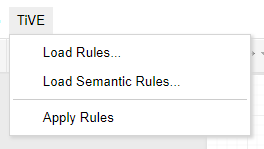
\includegraphics[]{Figure/tive_menu.PNG}
                \caption{Menu dei comandi per TiVE}
                \label{fig:tivemenu}
            \end{figure}

        \subsection{Riconoscimento grafo}
            All'interno di diagramma più simboli con scopi diversi possono condividere lo stesso elemento grafico creando delle ambiguità. Una delle prime fasi del processo di traduzione è il riconoscimento degli elementi e quindi la risoluzione di queste ambiguità. Come possiamo notare nella tabella~\ref{tab:final_syntax_definition}, in particolare nella seconda sotto-tabella, i connettori pur avendo uno scopo diverso condividono lo stesso elemento grafico, una linea.
            \newline
            Ancora, nella tabella \ref{tab:final_syntax_definition_tree} a condividere lo stesso elemento grafico è un simbolo: radice e nodo sono entrambi rappresentati da un cerchio.

            \begin{table}[htbp]
                \centering
                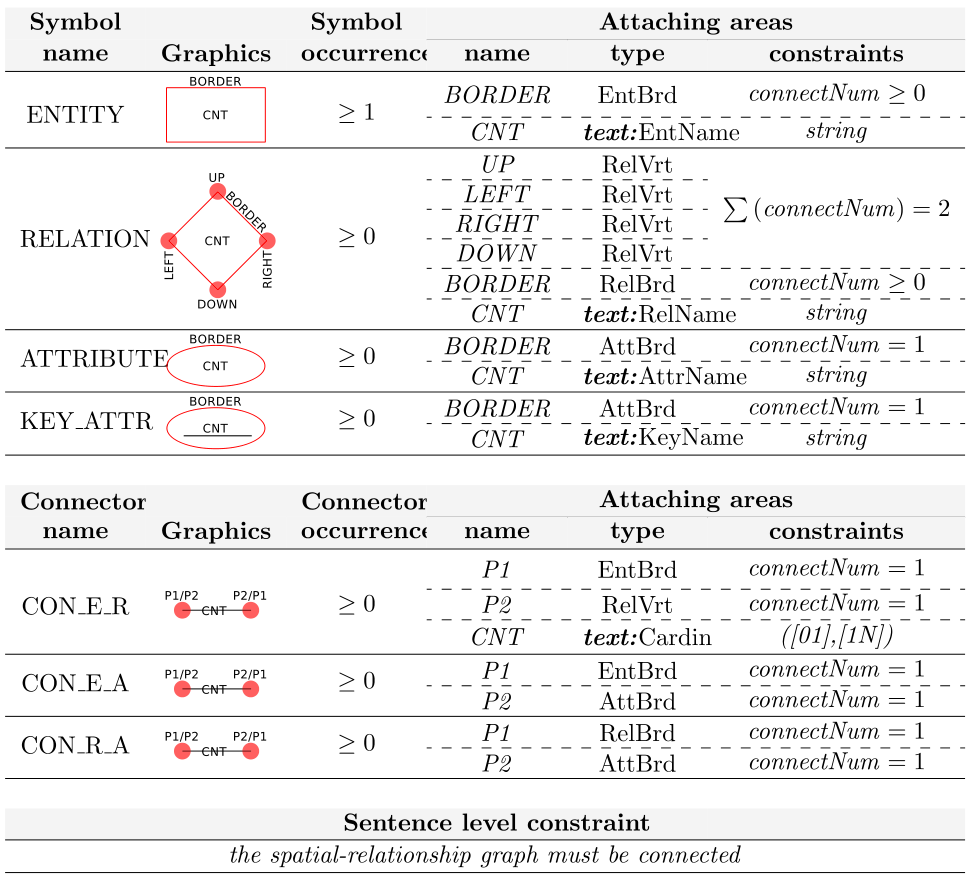
\includegraphics[scale=0.4]{Figure/final_syntax_definition.PNG}
                \caption{Specifica di un diagramma ER}
                \label{tab:final_syntax_definition}
            \end{table}

            \begin{table}[htbp]
                \centering
                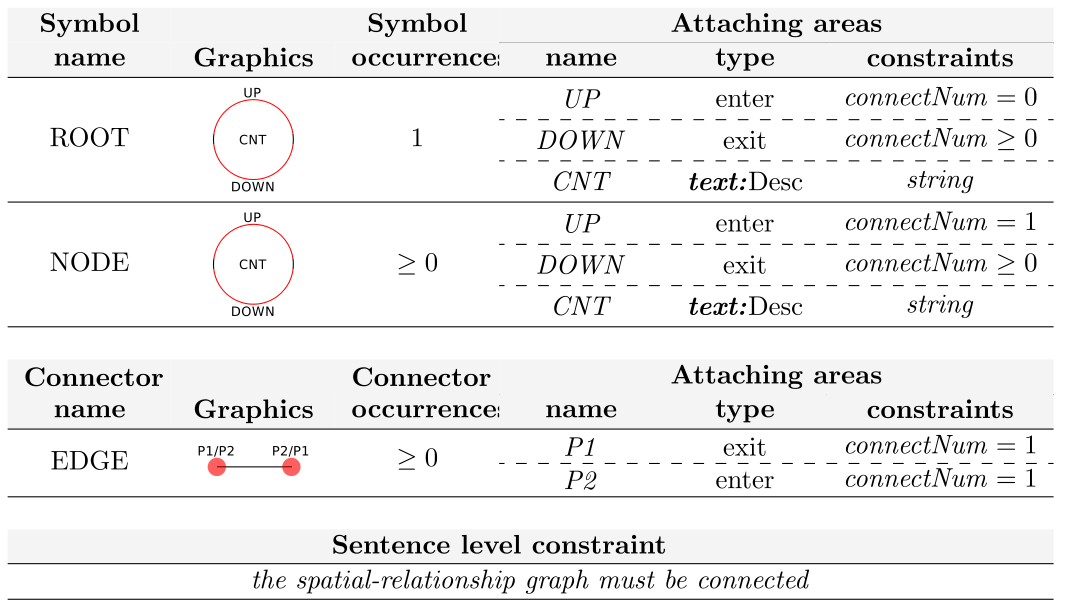
\includegraphics[scale=0.4]{Figure/final_syntax_definition_tree.PNG}
                \caption{Specifica di un Albero}
                \label{tab:final_syntax_definition_tree}
            \end{table}

            A caratterizzare un elemento sono le proprietà della definizione sintattica correlata. La disambiguazione viene effettuata tenendo in considerazione questi elementi.
            \newline
            L'algoritmo risolutivo innanzitutto rileva se si sta analizzando un vertice o un connettore e nel caso in cui venissero rivelate delle ambiguità procede come segue: Se l'elemento analizzato è un connettore prende in considerazione il campo \textit{Type} delle due aree d'attacco. All'interno di questa proprietà vengono indicati i tipi di area d'attacco in cui il connettore è collegato alle due estremità. Ad esempio, il connettore \textit{CON\_E\_A} (Connettore Entità-Attributo) alle due estremità si connetterà ad una \textit{EntBrd} e ad una \textit{AttBrd} in posizioni arbitrali; Nel caso un cui l'elemento analizzato è un vertice allora il controllo viene effettuato sui vincoli definiti per ogni simbolo. Il vertice sarà associato al simbolo per cui verranno rispettate tutti i suoi vincoli. Ad esempio, il simbolo \textit{Root} dovrà avere un numero di connessioni (\textit{connectNum}) uguali a zero sull'attaching area UP di tipo enter e un numero maggiore o uguale a zero di connessioni sull'attaching area DOWN di tipo exit.
            \newline

        \subsection{Applicazione definizioni}
            Eseguito il riconoscimento di ogni simbolo appartenente al grafo si può procedere con l'applicazione delle definizioni. Come ho già accennato, la specifica delle definizioni si divide in due parti: sintattica e semantica.

            \subsubsection{Definizioni Sintattiche}
                Ogni linguaggio ha delle regole sintattiche da rispettare. Un esempio di definizione sintattica è raffigurata nella tabella \ref{tab:final_syntax_definition}. Nella colonna \textit{Symbol occurences} vi è un vincolo al livello del simbolo, indica quante occorrenze del simbolo devono essere presenti all'interno del diagramma. Nell'ultima colonna, \textit{constraints}, vi troviamo i vincoli al livello degli Attaching Point e il formato che deve avere il campo di testo dell'elemento se specificato. Nell'ultima riga, \textit{Sentence level constraint}, troviamo i vincoli che il diagramma deve rispettare.
                \newline
                Come ho già accennato, in Tive le definizioni erano scritte in formato XML (vedi Appendice \ref{appendix:xml_definition}). Successivamente sono state implementate in formato JSON\footnote{JavaScript Object Notation} per poter essere interpretate in maniera nativa dal linguaggio di programmazione usato. All'interno dello snippet di codice \ref{lst:newDefinition} vi è una parte della definizione nel nuovo formato. 
                \newline
                Il valore di "\textit{ap}" è un array contenente i vincoli per i punti d'attacco; "\textit{text}" contiene le informazioni riguardanti le aree di testo, "\textit{\_name}" è il nome del simbolo; "\textit{\_ref}" indica a quale figura grafica si fa riferimento; "\textit{occurences}" è il vincolo sulle occorrenze del simbolo.
                \newline
                L'intera definizione è consultabile all'Appendice \ref{appendix:jsonDefinition}.
                \begin{spacing}{0.5}
                    \lstinputlisting[language=JavaScript, caption={\textbf{Frammento della definizione sintattica in formato JSON di un linguaggio, nel particolare la specifica per il simbolo \textit{ROOT} (o Radice).}},label={lst:newDefinition}, firstline=4, lastline=29]{SourceCode/newDefinition.json}
                \end{spacing}

            \subsubsection{Definizioni Semantiche}
                Le definizioni semantiche sono necessarie alla traduzione del diagramma. Un esempio di definizione semantica (o definizione LCSD) è raffigurata nella tabella \ref{tab:semantic_specification}. Come già detto nella sezione \ref{sec:semantica} la specifica semantica è composta da quattro elementi fondamentali: \textit{Property} indica il nome della proprietà semantica da attribuire all'elemento della specifica; \textit{Procedure} è il nome della procedura da utilizzare per assegnare o modificare la proprietà; \textit{Params} sono i parametri da passare alla procedura; \textit{Post-condition} è la condizione che deve essere rispettata al termine dell'esecuzione della procedura.
                \newline
                Anche in questo caso, le definizioni sintattiche sono state trascritte dal formato XML al formato JSON. All'interno dello snippet di codice \ref{lst:newSemanticDefinition} vi è una parte della definizione nel nuovo formato. 
                \newline
                Il valore di "\textit{property}" contiene tutte le proprietà da computare; Ogni proprietà è composta dai seguenti componenti: "\textit{\_name}" è il nome della proprietà; "\textit{\_type}" è il formato della proprietà; "\textit{procedure}" contiene le procedure da eseguire, ogni procedura è composta da: "\textit{\_postCondition}" è la condizione da rispettare al termine della procedura, "\textit{name}" è il nome della procedura, "\textit{\_path}" insieme a "\textit{\_param}" sono i parametri da passare alla procedura. Il campo "\textit{visit}" verrà utilizzato dall'algoritmo di ordinamento del grafo.
                \newline
                L'intera definizione è consultabile all'Appendice \ref{appendix:ERjsonSemanticDefinition}.
                \begin{spacing}{0.5}
                    \lstinputlisting[language=JavaScript, caption={\textbf{Frammento della definizione semantica in formato JSON di un linguaggio, nel particolare la specifica per il simbolo STAT}},label={lst:newSemanticDefinition}, firstline=200, lastline=241]{SourceCode/EXAMPLES/flowchartp/newSemanticDefinition.json}
                \end{spacing}

        \subsection{Applicazione Regole Semantiche}
            Se l'applicazione delle definizioni è andata a buon fine, l'algoritmo procede con il calcolo delle regole semantiche. La procedura si suddivide in due fasi: ordinamento del grafo e calcolo delle definizioni semantiche.

            \subsubsection{Ordinamento del grafo}
                In precedenza ho parlato del campo "\textit{visit}" presente all'interno della definizione semantica di un linguaggio. Questo campo serve a costruire una "Visit Table" necessaria a definire l'ordine in cui gli elementi del diagramma verranno visitati.

                \begin{table}[htbp]
                    \centering
                    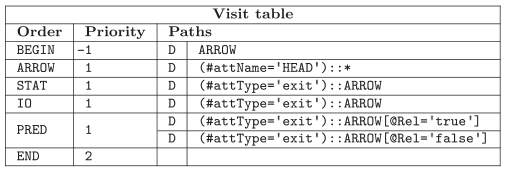
\includegraphics[scale=0.6]{Figure/visitTable.PNG}
                    \caption{Visit Table per il linguaggio Flowchart}
                    \label{tab:visitTable}
                \end{table}

                Ogni simbolo ha una priorità, come mostrato nella tabella \ref{tab:visitTable}. Questa tabella specifica la priorità per ogni elemento del linguaggio flowchart, in particolare -1 per il simbolo BEGIN, 2 per il simbolo END e 1 per tutti gli altri simboli. In questo modo il simbolo BEGIN verrà posizionato all'inizio, END alla fine e gli altri simboli in una posizione arbitraria. 
                \newline
                La colonna "Paths" della tabella indica il prossimo nodo da esplorare, se presente. E' composta da due sezioni, una è un flag che indica se l'esplorazione viene effettuata in ampiezza (B) o un profondità (D).
                \newline
                Altro modo di definire un ordine è con la "Path Table", mostrata nella tabella \ref{tab:pathTable}. 

                \begin{table}[htbp]
                    \centering
                    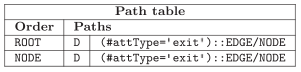
\includegraphics[scale=0.85]{Figure/pathTable.PNG}
                    \caption{Path Table per il linguaggio Tree}
                    \label{tab:pathTable}
                \end{table}

                La tabella di visita viene applicata al diagramma dalla funzione \texttt{ApplyVisitTable} (snippet \ref{lst:applyVisitTable}) che fa uso di un'altra funzione fondamentale, \texttt{FollowPath} (snippet \ref{lst:followPath}).

                \begin{lstlisting}[language=JavaScript, basicstyle=\tiny, caption={La funzione applyVisitTable}, label={lst:applyVisitTable}]
                    /**
                    * Apply the visit table to the graph
                    */
                    CheckUtil.prototype.applyVisitTable = function (graph, visitTable) {
                        let N = Object.values(graph).sort((a, b) => {
                            return visitTable[a.name].order - visitTable[b.name].order;
                        });

                        let L = [];
                        while (N.length != 0) {
                            let rem = N.shift();
                            L.push(rem);

                            let nodes = [];
                            nodes = this.followPath(rem, graph, N, visitTable, nodes);
                            L = L.concat(nodes);

                            N = N.filter((i) => {
                                return nodes.indexOf(i) < 0;
                            });

                        }

                        L = this.stableSort(L, (a, b) => {
                            if (visitTable[a.name].priority > visitTable[b.name].priority) {
                                return 1;
                            }
                            if (visitTable[a.name].priority < visitTable[b.name].priority) {
                                return -1;
                            }
                        });
                        return L;
                    }
                \end{lstlisting}

                \begin{lstlisting}[language=JavaScript, basicstyle=\tiny, caption={La funzione followPath}, label={lst:followPath}]
                    /**
                    * Follow the path from a node
                    */
                    CheckUtil.prototype.followPath = function (node, G, N, PTPATHS, nodes) {
                        let nname = node.name;
                        let npaths = PTPATHS[nname].paths;
                        for (let elem in npaths) {
                            let npath = npaths[elem];
                            let nds = this.resolvePath(node, npath._value);
                            nds = nds.filter((i) => {
                                return nodes.indexOf(i) < 0;
                            });
                            nds = nds.filter((i) => {
                                return N.indexOf(i) > -1;
                            });

                            if (npath._flag == 'B') {
                                nodes = nodes.concat(nds);
                            }
                            for (let elem in nds) {
                                let n = nds[elem];
                                if (npath._flag == 'D') {
                                    if (nodes.indexOf(n) < 0) {
                                        nodes.push(n);
                                    }
                                }
                                nodes = this.followPath(n, G, N, PTPATHS, nodes);
                            }
                        }
                        return nodes;
                    }
                \end{lstlisting}

                Ordinato il grafo, l'algoritmo procede con l'applucazione delle definizioni semantiche.
                
            \subsubsection{Calcolo definizioni semantiche}
                Altro ruolo importante è della funzione \texttt{ApplySemanticRules} (snippet \ref{lst:applySemanticRules}).

                \begin{lstlisting}[language=JavaScript, basicstyle=\tiny, caption={La funzione che computa tutte le proprietà semantiche}, label={lst:applySemanticRules}]
                    /**
                    * Apply the semantic rules to the graph
                    */
                    CheckUtil.prototype.applySemanticRules = function (graph, semanticRules) {

                        let completedNodes = [];

                        // DELETING ALL THE NODES WHICH AREN'T SEMANTIC RULES
                        for (let elem in graph) {
                            let graphElem = graph[elem];
                            let graphElemSemRule = semanticRules[graphElem.name];
                            if (!graphElemSemRule) {
                                delete graph[elem];
                            }
                        }

                        graph = graph.filter((el) => {
                            return el != null;
                        });

                        let loop = 0;

                        while (!graph.length == 0) {

                            if (++loop == 100) {
                                console.log('loop');
                                break;
                            }

                            for (let elem in graph) {

                                let x = graph[elem];
                                let xRules = semanticRules[x.name];
                                let propertyToCalculate = xRules.property.length;
                                let calculatedProperties = this.calculateProperties(x, xRules);
                                console.log("CALCULATED: " + calculatedProperties);
                                console.log("TO CALCULATE: " + propertyToCalculate);
                                if (propertyToCalculate == calculatedProperties) {
                                    x.status = "COMPLETE";
                                    completedNodes.push(x);
                                } else {
                                    x.status = "INCOMPLETE";
                                }
                            }
                            console.info('COMPLETED NODES: ', completedNodes);
                            graph = graph.filter((i) => {
                                return completedNodes.indexOf(i) < 0;
                            });
                            console.info('INCOMPLETED NODES: ', graph);
                        }
                        return true;
                    }
                \end{lstlisting}

                Come possiamo notare dal codice, l'algoritmo prende in input il grafo resituito dalla funzione \texttt{applyVisitTable} (\ref{lst:applyVisitTable}) e le regole semantiche, ad esempio \ref{appendix:jsonSemanticDefinition} o \ref{appendix:ERjsonSemanticDefinition}.
                L'algoritmo analizza ogni simbolo e gli assegna lo status "COMPLETE" solo se sono state calcolate tutte le proprietà compresa l'azione. Lo stesso simbolo può essere analizzato più volte fin quando non vengono calcolate tutte le proprietà definite all'interno delle regole semantiche. Per evitare la creazione di deadlock\footnote{In questo caso si verifica una deadlock se la computazione delle proprietà di uno o più simboli creano uno stallo} è stata inserita una variabile \texttt{"loop"} che farà arrestare l'algoritmo se viene raggiunto un numero alto di iterazioni senza terminare il calcolo di tutte le proprietà.
                \newline
                Una volta applicate le definizioni, TiveJS mostrerà all'interno di una Console la traduzione semantica del diagramma (figura \ref{fig:semanticTranslation}) se non ci sono errori, altrimenti mostrerà all'interno della console gli errori che si sono verificati. Inoltre gli elementi coinvolti in quel errore saranno evidenziati in rosso, figura \ref{fig:semanticTranslation_error}.
                \begin{figure}[htbp]
                    \centering
                    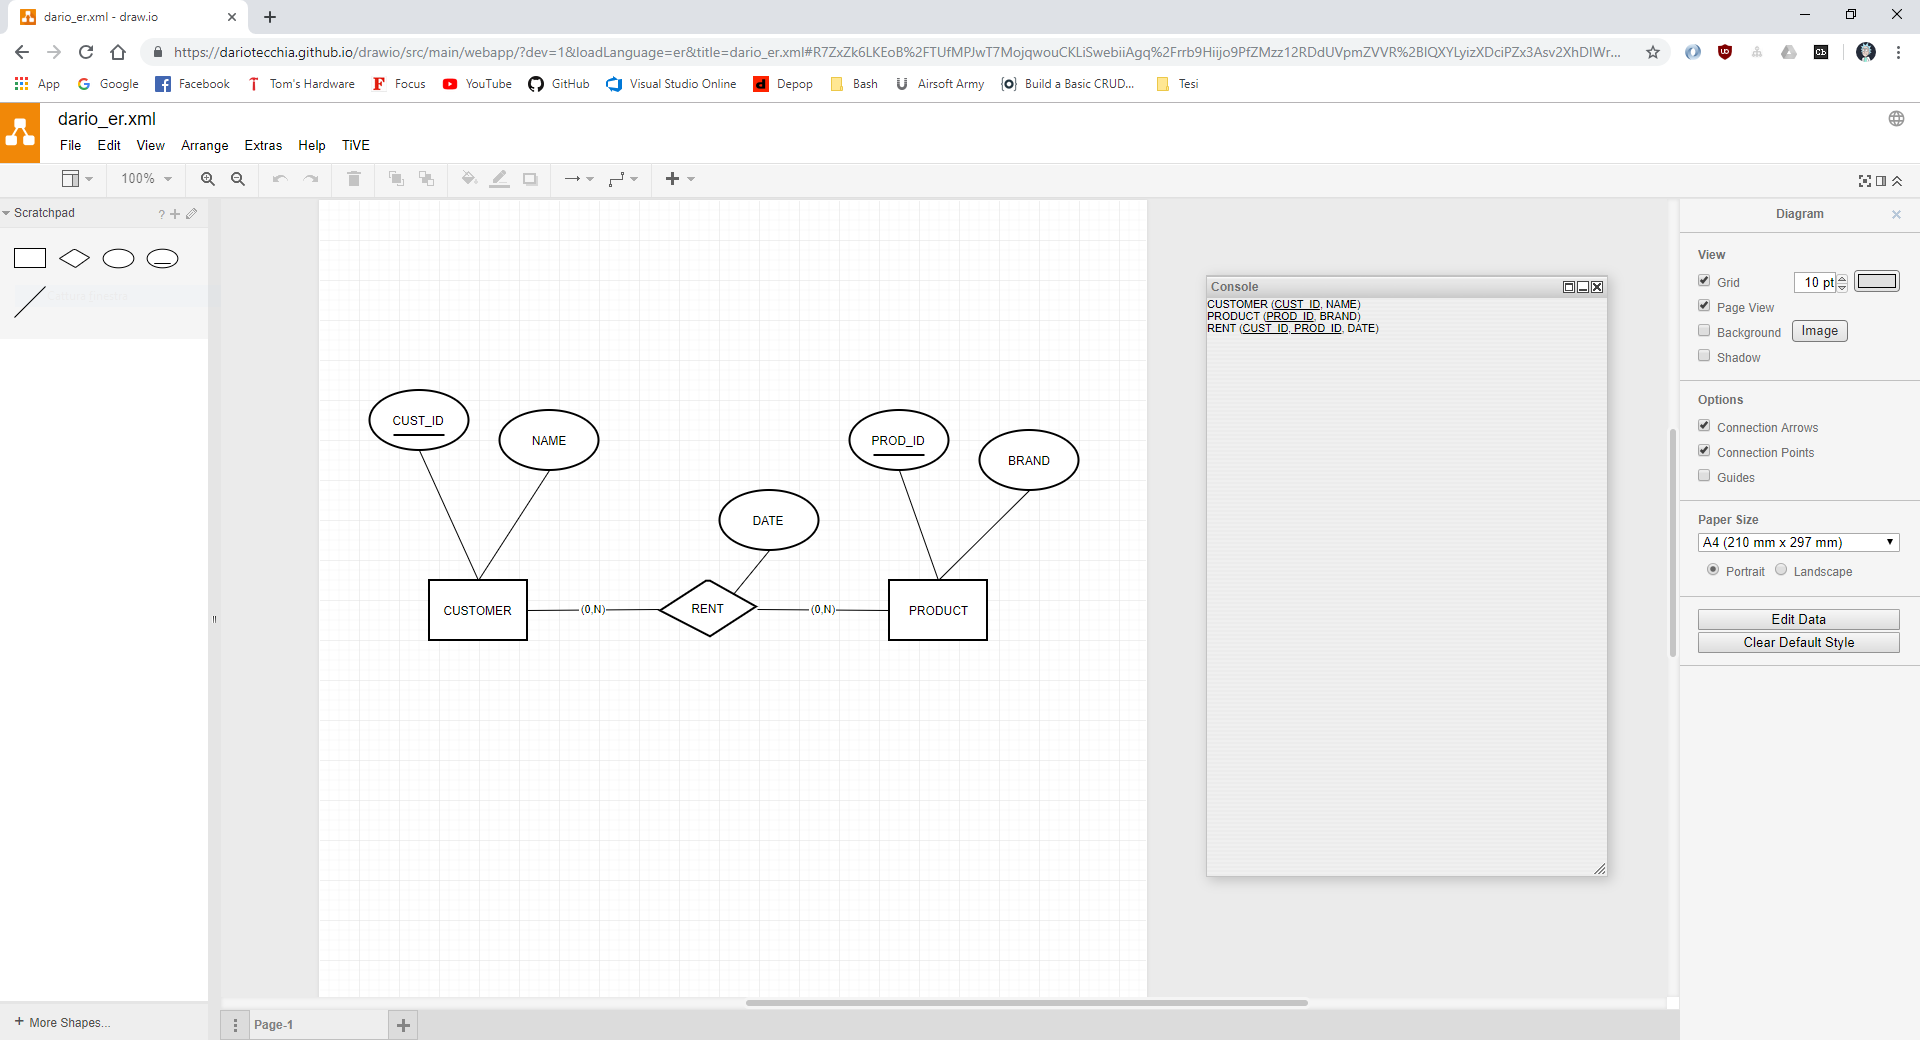
\includegraphics[scale=0.20]{Figure/semanticTranslation.PNG}
                    \caption{TiveJS con la traduzione semantica di un diagramma entità\-relazione mostrata in una console (sulla destra)}
                    \label{fig:semanticTranslation}
                \end{figure}

                \begin{figure}[htbp]
                    \centering
                    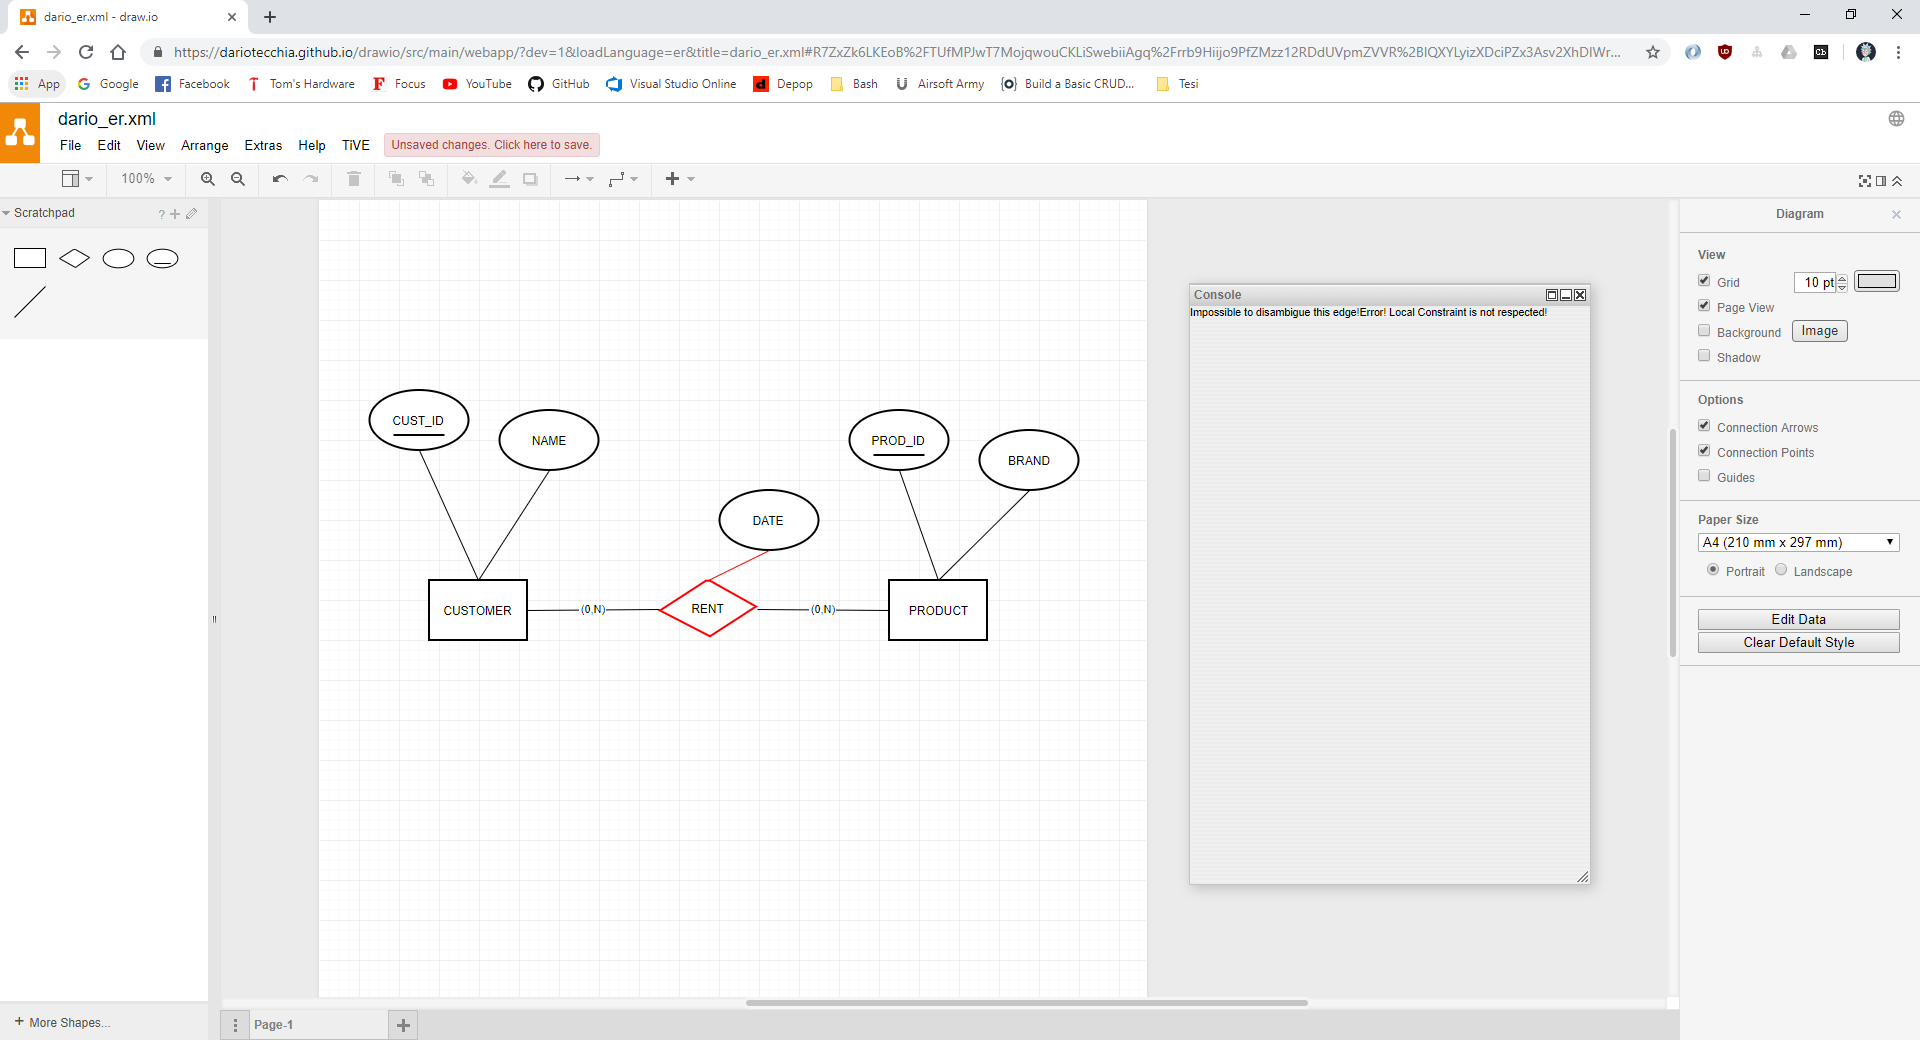
\includegraphics[scale=0.20]{Figure/semanticTranslation_error.PNG}
                    \caption{TiveJS con gli errori mostrati in una console (sulla destra)}
                    \label{fig:semanticTranslation_error}
                \end{figure}

    \section{Tecnologie Utilizzate: JavaScript}
        TiveJS è stata implementata completamente in JavaScript per far si che potesse girare su ogni browser web.
        JavaScript, a volte abbreviato con JS, è un linguaggio di programmazione interpretato ad alto livello. Standardizzato per la prima volta nel 1997 con il nome di ECMAScript (attualmente l'ultima release è ECMAScript 2018~\cite{ecmascript}), insieme all'HTML e il CSS è una delle tecnologie alla base del World Wide Web.
        In questa sezione esaminiamo alcuni dei punti di forza di JavaScript, così da capire quali sono le sue particolarità.

        \subsection{Punti di Forza di JavaScript}

            \subsubsection{Ricco di librerie}
                JavaScript, oltre le sue librerie standard, conta un numero impressionante di librerie scritte da una community molto attiva. Dispone di API per lavorare con testo, matrici, date, espressioni regolari e DOM\footnote{Document Object Model}.

            \subsubsection{Supporto universale}
                Tutti i moderni browser web supportano nativamente JavaScript con gli interpreti implementati al loro interno.
            
            \subsubsection{Multi-paradigma}
                JavaScript è un linguaggio multi-paradigma, che supporta la programmazione basata sugli eventi, la programmazione funzionale e quella imperativa (inclusa la programmazione orientata agli ogetti).

            \subsubsection{Portabile}
                JavaScript è un linguaggio portabile. E' possibile usarlo su diverse piattaforme come: \textit{Linux, Windows, OSx, iOS e Android}. Questo è possibile perchè non dipende dalla macchina dove gira essendo interpretato e non compilato. E' necessario però un interprete JavaScript.

            \subsubsection{Semplice}
                Molto semplice da imparare e perfetto da usare come linguaggio accademico essendo ad un linguaggio ad alto livello.

            \subsubsection{Gratis}
                JavaScript è totalmente gratis ed è possibile utilizzarlo e distribuirlo senza restrizioni di copyright. Nonostante questo, alle spalle ha una community attivissima.

        \subsection{Principali Applicazioni}
            Pur essendo un linguaggio rilasciato per i browser web, Netscape, nel 1995 introdusse una nuova implementazione del linguaggio per lo scripting server-side. Una delle implementazioni server-side più famosa è Node.js.

        \section{Librerie utilizzate nel Progetto}
            \subsubsection{mxGraph}
                Come accennato, una delle librerie utilizzate all'interno di TiveJS è mxGraph. Serve per lo sviluppo di diagrammi e permette la creazione di applicazioni interattive per la creazione di grafi e diagrammi. Oltre che in JavaScript è scritta anche in linguaggi server side quali PHP, .NET e Java~\cite{mxgraph}.
            \subsubsection{jQuery}
                jQuery risulta essere la libreria JavaScript più utilizzata su Internet per via della facilità di installazione e utilizzo.
                \newline
                Lo slogan di jQuery non a caso è \textit{<<write less, do more>>} poichè nasce con l'intenzione di semplificare la selezione, la manipolazione, la gestione degli eventi e l'animazione di elementi DOM in pagine HTML, nonchè implementare funzionalità AJAX~\cite{jquery}.
                \newline
                Da agli sviluppatori un'interfaccia semplice, accessibile attraverso il caratteristico simbolo \textbf{\$}, astraendo comandi molto più complessi offerti da JavaScript. E' un software libero.